\subsection{Algorithmus}\label{subsec:algorithmus}

\paragraph{AVL-Bedingung}
Ein AVL-Baum ist ein Binärbaum, der die zusätzliche Eigenschaft besitzt, dass
die Balance, die als die Differenz der Höhe $h$ der beiden
Teilbäume definiert ist (siehe Formel~\ref{eq:balance}), bei jedem Knoten mindestens 1 und
maximal 1 beträgt.
Diese Eigenschaft wird AVL-Bedingung genannt.
Dabei ist die Höhe analog zum regulären Binärbaum definiert (siehe Formel~\ref{eq:height}).

\begin{equation}
    bal(k) = h(T_r) - h(T_l)\label{eq:balance} \in \{-1,0,1\}
\end{equation}
\begin{equation}
    h(k) = max(h(T_l), h(T_r))\label{eq:height}
\end{equation}
Durch diese Bedingung wird sichergestellt, dass der Baum zu jedem Zeitpunkt
balanciert ist und somit das in der Einleitung beschriebene Problem der
schlechten Laufzeit des Binärbaumes durch Entartung nicht auftreten kann.

\paragraph{Rebalancierung}\label{par:rebalancing}
Nach dem Einfügen und Löschen von Elementen kann es jeweils vorkommen, dass die
Balance eines Konten -2 oder 2 beträgt.
Somit muss der AVL-Baum nach diesen Operationen die AVL-Bedingung überprüfen,
und eventuell eine Rebalancierung vornehmen.
Dabei wird zwischen insgesamt vier Fällen unterschieden, die durch die Folge
der Balancewerte definiert sind (siehe auch Abbildung~\ref{fig:AVL-Cases}):
\begin{enumerate}
    \item Left Left: -2/-1 oder -2/0 → Rechtsrotation\label{enm:rebal1}
    \item Right Right: +2/+1 oder +2/0 → Linksrotation \label{enm:rebal2}
    \item Left Right: -2/+1 → Doppelte Rechtsrotation \label{enm:rebal3}
    \item Right Left: +2/-1 → Doppelte Linksrotation \label{enm:rebal4}
\end{enumerate}
Die ersten beiden und letzten beiden Fälle sind dabei jeweils symmetrisch zueinander.

\paragraph*{Rotation}\label{par:rotating}

Die Rebalancierung wird mithilfe von Rotationen von Knoten vorgenommen.
Bei einer Rotation wird immer ein Knoten als Wurzelknoten betrachtet.
Alle Knoten, die über dem Wurzelknoten stehen, sind für die Rotation nicht von
Relevanz.
%Im Left Left bzw. Right Right Case ist dies der Knoten,
%bei dem die AVL-Bedingung verletzt wird.
Der Wurzelknoten wird mit dem Kindknoten rotiert, auf dessen Seite die
Unbalance vorliegt, im Folgenden wird dieses Kind Rotationsknoten genannt:
\begin{itemize}
    \item Linksrotation: Rotieren vom Wurzelknoten mit rechtem Kindknoten
    \item Rechtsrotation: Rotieren vom Wurzelknoten mit linken Kindknoten
\end{itemize}
Betrachte Abbildung~\ref{fig:AVL-Cases}~(Left~Left~Case).
Zum Rotieren der beiden Knoten nach rechts werden folgende Operationen ausgeführt:
\begin{enumerate}
    \item Der Wurzelknoten (5) wird als rechtes Kind vom Rotationsknoten (4)
    gesetzt\label{enm:reblStep1}
    \item Der eben ersetzte Knoten (C) (rechtes Kind vom Rotationsknoten) wird als linkes Kind
    des ursprünglichen Wurzelknotens (5) gesetzt\label{enm:reblStep2}
    \item Der Rotationsknoten (4) wird als neue Wurzel gesetzt\label{enm:reblStep3}
\end{enumerate}
Dabei muss die Höhe des Rotations- und Wurzelknotens angepasst werden.
Dies lässt sich am leichtesten durch eine erneute Berechnung mit Formel~\ref{eq:height} erzielen.
Des Weiteren muss eventuell die Höhe der Knoten über dem Wurzelknoten angepasst werden.

An Abbildung~\ref{fig:AVL-Cases}~(Balanced) wird deutlich, dass durch die
Rechtsrotation beim Left Left Case die AVL-Bedingung wieder erfüllt ist.

Eine Linksrotation erfolgt symmetrisch.

\paragraph{Doppelrotation}

Bei den Fällen Left Left und Right Right konnte der Baum mit lediglich
einer Rotation balanciert werden.
Dies reicht bei den anderen Fällen nicht aus, wie wird aus Abbildung~\ref{fig:AVL-wrong-rotate}
ersichtlich wird.

Es müssen insgesamt zwei Rotationen durchgeführt werden:
Mit der ersten Rotation wird der Left Left bzw. Right Right Case
herbeigeführt, die zweite Rotation befriedigt anschließen die AVL-Bedingung.
Betrachte Abbildung~\ref{fig:AVL-Cases} (Left Right Case).
Im Left Right Case wird zunächst eine Linksrotation zwischen dem linken
Kindknoten des Wurzelelementes und des rechten Nachfolgers ausgeführt.
Diese Rotation wird symmetrisch zur oben beschriebenen Rechtsrotation ausgeführt.
Anschließend liegt der Left Left Case vor, eine einfache Rechtsrotation
befriedigt nun die AVL-Bedingung.


\begin{figure}[hbt]
    \centering
    %https://fr.m.wikipedia.org/wiki/Fichier:AVL_Tree_Rebalancing.svg
    %https://github.com/LambdaSchool/Data-Structures
    %https://commons.wikimedia.org/wiki/File:AVL_Tree_Rebalancing_he.svg
    \begin{minipage}[c]{.45\textwidth}
    \subfloat[Korrekt]{
        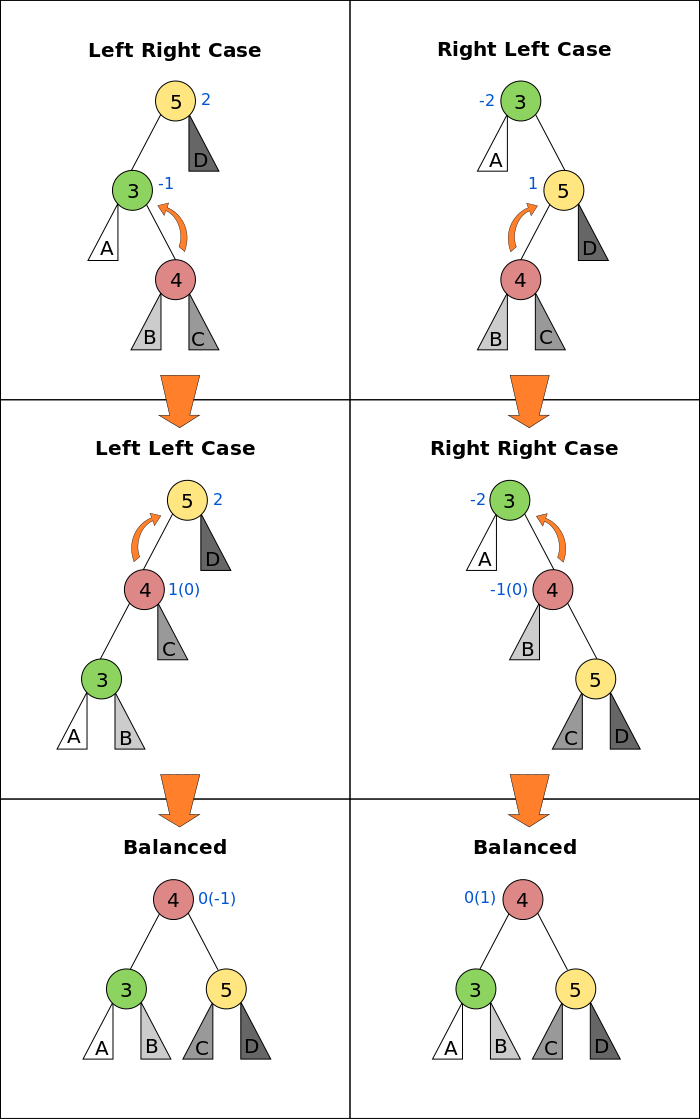
\includegraphics[width=.95\linewidth]{img/external/AVL_Tree_Rebalancing}
        \label{fig:AVL-Cases}}
    \end{minipage}
    \begin{minipage}[c]{.45\textwidth}
    \subfloat[Falsch]{
        \includegraphics[width=.95\linewidth]{img/external/AVL_Tree_Rebalancing_wrong.pdf}
        \label{fig:AVL-wrong-rotate}}
    \end{minipage}
    \caption{Rebalancierung}
\end{figure}
%\begin{figure}[hbt]
%    \centering
%    \includegraphics[width= 0.45\textwidth]{img/AVL_Tree_Rebalancing_wrong.pdf}
%    \caption{Falsche Rotation}
%\end{figure}

\subsection{Entwurf}\label{subsec:entwurf2}

\paragraph{InitBT, IsEmptyBT, EqualBT, FindBT}
Die Implementation dieser Methoden kann aus der Implementation des Binärbaumes übernommen werden.
Bei der InitBT Methode müssen lediglich alle Counter der Rotationszählung zurückgesetzt werden.

\paragraph{IsBT}\label{par:avl-isBT}
Die Methode von dem Binärbaum wird um die Überprüfung der AVL-Bedingung erweitert.
Dabei wird bei jedem Knoten zusätzlich überprüft, ob die Balance (siehe Formel~\ref{eq:balance})
-1, 0 oder +1 beträgt.
Der Ausdruck wird mit den bisherigen Ausdrücken und-verknüpft.

\paragraph{InsertBT, DeleteBT}
Das Einfügen und Löschen wird wie bei einem Binärbaum realisiert.
Die einzige Änderung, die vorgenommen werden muss, ist das Prüfen der
AVL-Bedingung und eventuelles Rotieren, bottom-up nach dem Einfügen bzw. Löschen.
Dies wird mithilfe der \verb|Rebalance|-Methode vorgenommen, die in
Abschnitt~\nameref{par:MethodRebalance} weiter ausgeführt wird.
Beim Löschen muss darauf geachtet werden, dass der Pfad vom tatsächlich entfernten Knoten, also
dem Substitution-Knoten, überprüft wird.
In Abbildung~\ref{fig:AVL-insert} und~\ref{fig:AVL-delete} sind die notwendigen Änderungen jeweils
blau markiert.

\begin{figure}[htbp]
    \centering
    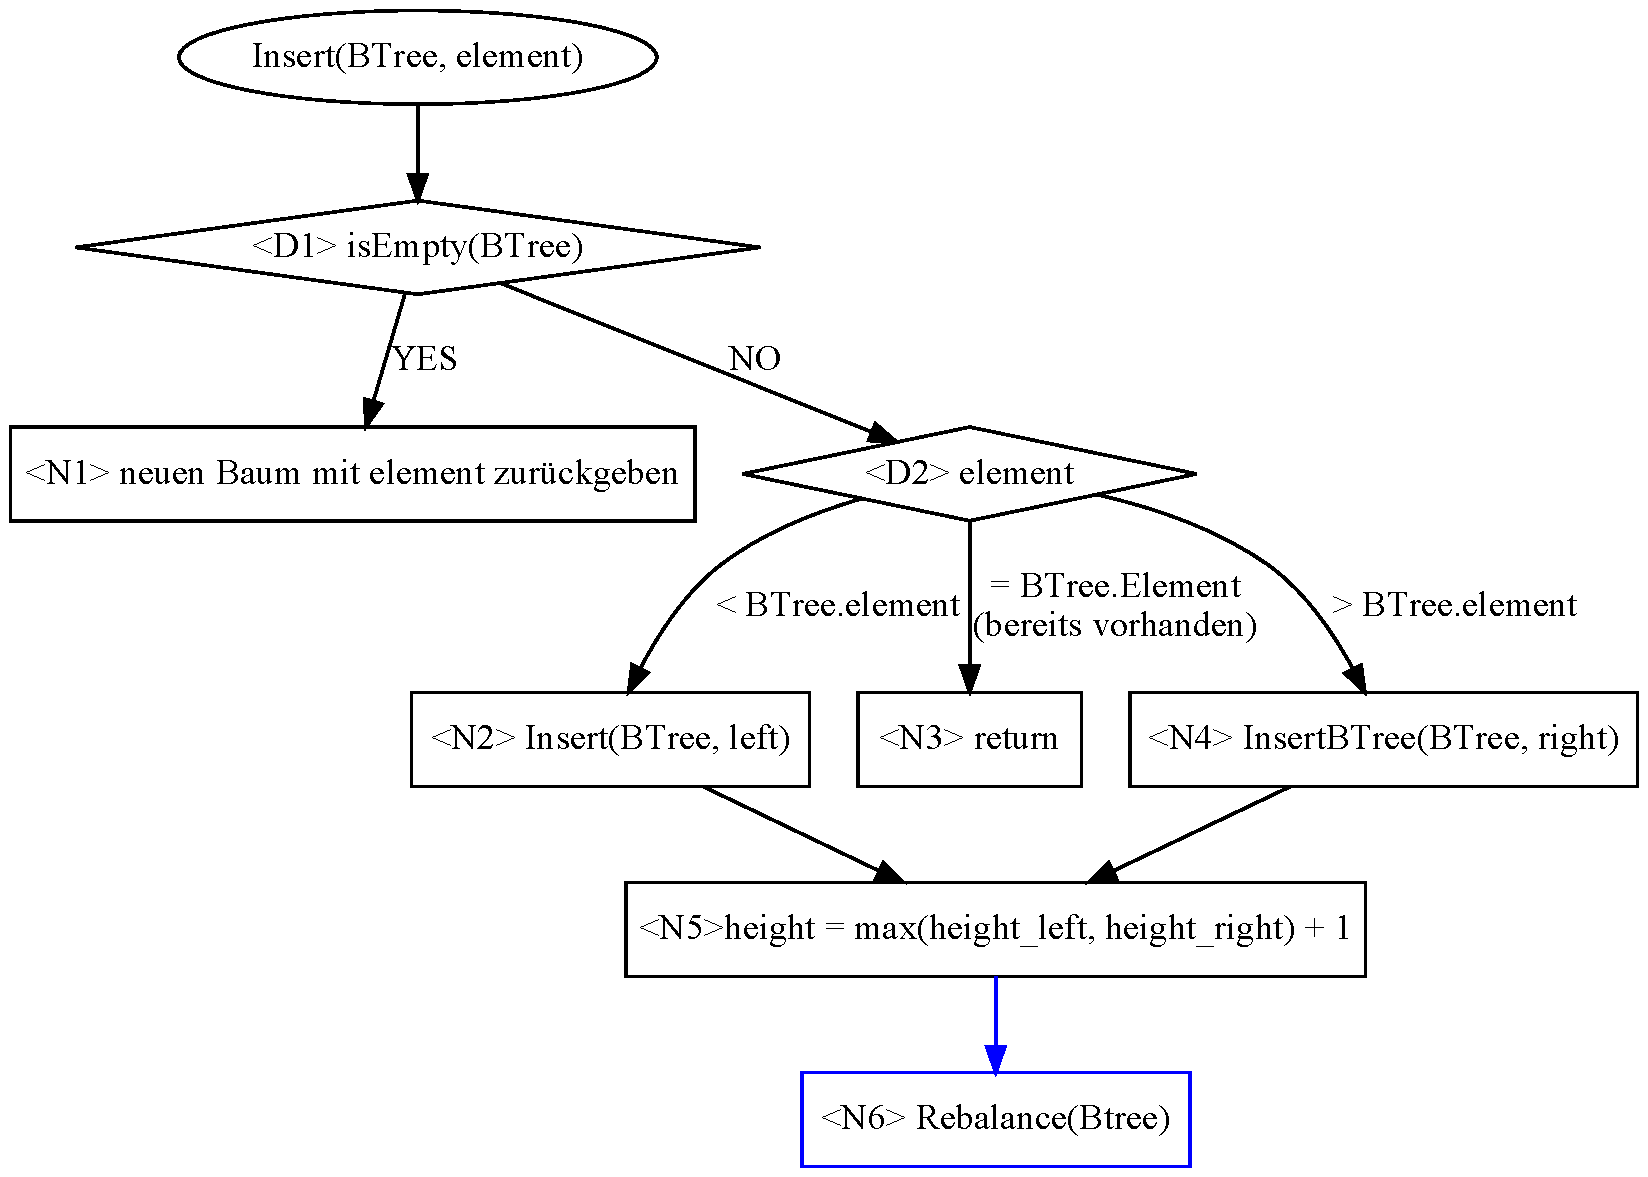
\includegraphics[width= 0.70\textwidth]{img/gv/insert}
    \caption{InsertBT}
    \label{fig:AVL-insert}
\end{figure}
\begin{figure}[p]
    \centering
    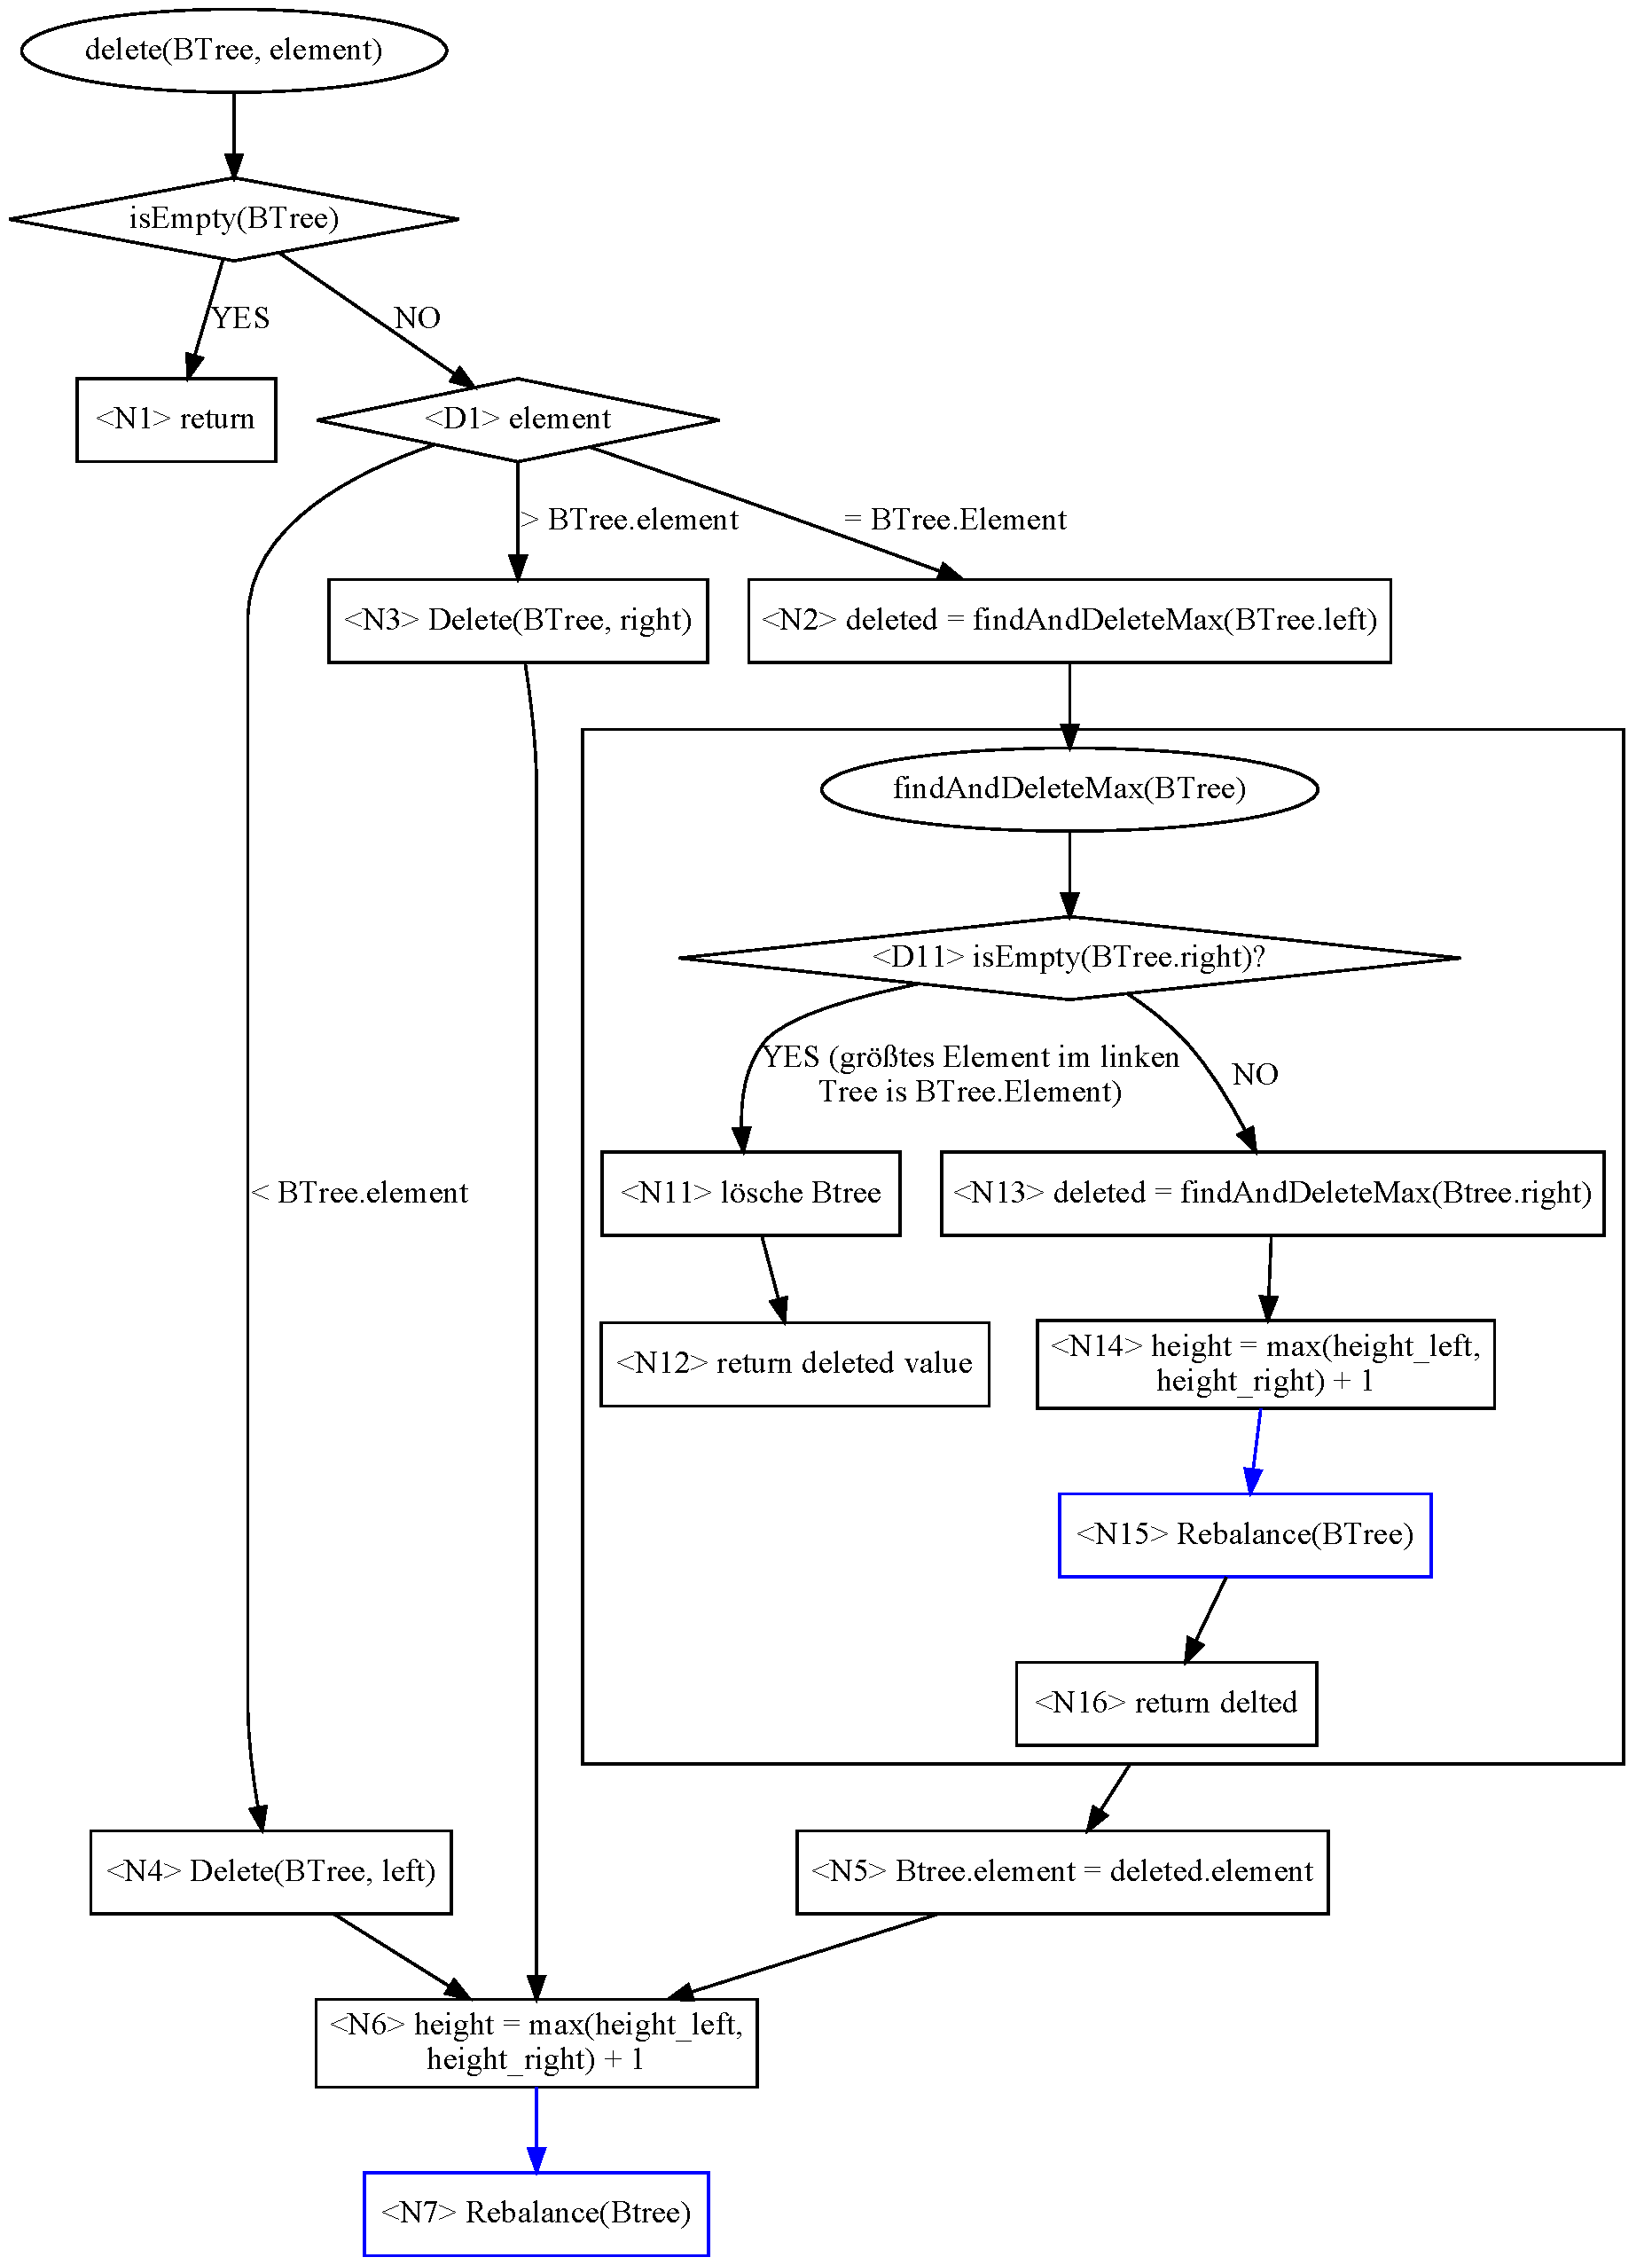
\includegraphics[height= 0.97\textheight]{img/gv/delete}
    \caption{DeleteBT}
    \label{fig:AVL-delete}
\end{figure}

\paragraph{PrintBT}\label{par:printBT}
Diese Funktion speichert eine Representation des übergebenen Baumes als Datei im GraphViz Format.
Dafür wird am Anfang einmal der Header (\verb|digraph G{|), dann der Inhalt, am Ende eine
schließende Klammer ausgegeben.
Um den Inhalt auszugeben werden für jeden Knoten bis zu drei Zeilen ausgegeben:
\begin{enumerate}
    \item \verb|<Knoten> -> <Linkes Kind>;|
    \item \verb|<Knoten> -> <Rechtes Kind>;|
    \item \verb|<Knoten> [label = "<Knoten>\n(<Hoehe von Knoten>)" color = <Farbe>];|
\end{enumerate}
Dabei entspricht \verb|Knoten, Linkes Kind, Rechtes Kind| dem Wert des jeweiligen Knotens.
Falls ein Kindknoten leer sein sollte, wird dafür nur die letzte Zeile ausgegeben.
Diese formatiert den Knoten selber, dabei wird die Farbe abhängig der Balance gesetzt.

Knoten mit der Balance von \(-1\) werden violett, mit der Balance von \(+1\)
blau, mit der Balance von \(0\) schwarz dargestellt.
Falls die AVL-Bedingung nicht eingehalten wird, erscheint der Knoten rot.

\paragraph{Rebalance}\label{par:MethodRebalance}
Die \verb|Rebalance|-Methode bekommt einen Knoten übergeben, überprüft die AVL-Bedingung und
balanciert den Knoten durch Rotieren, falls die AVL-Bedingung nicht erfüllt ist.
Dafür wird zunächst die Balance des übergebenen Knotens überprüft.
Falls diese -1, 0, +1 beträgt, wird der Knoten nicht verändert.
Andernfalls wird überprüft, welcher der in Abschnitt \nameref{par:rebalancing} aufgeführten Fälle
vorliegt und die nötigen Rotationen mithilfe der \nameref{par:MethodRotate}-Methode ausgeführt.
Falls eine Doppelrotation ausgeführt wird, wird außerdem der entsprechende Counter erhöht.
In Abbildung~\ref{fig:rebalance} wird die Methode in einem Flussdiagramm dargestellt.
\begin{figure}[p]
    \centering
    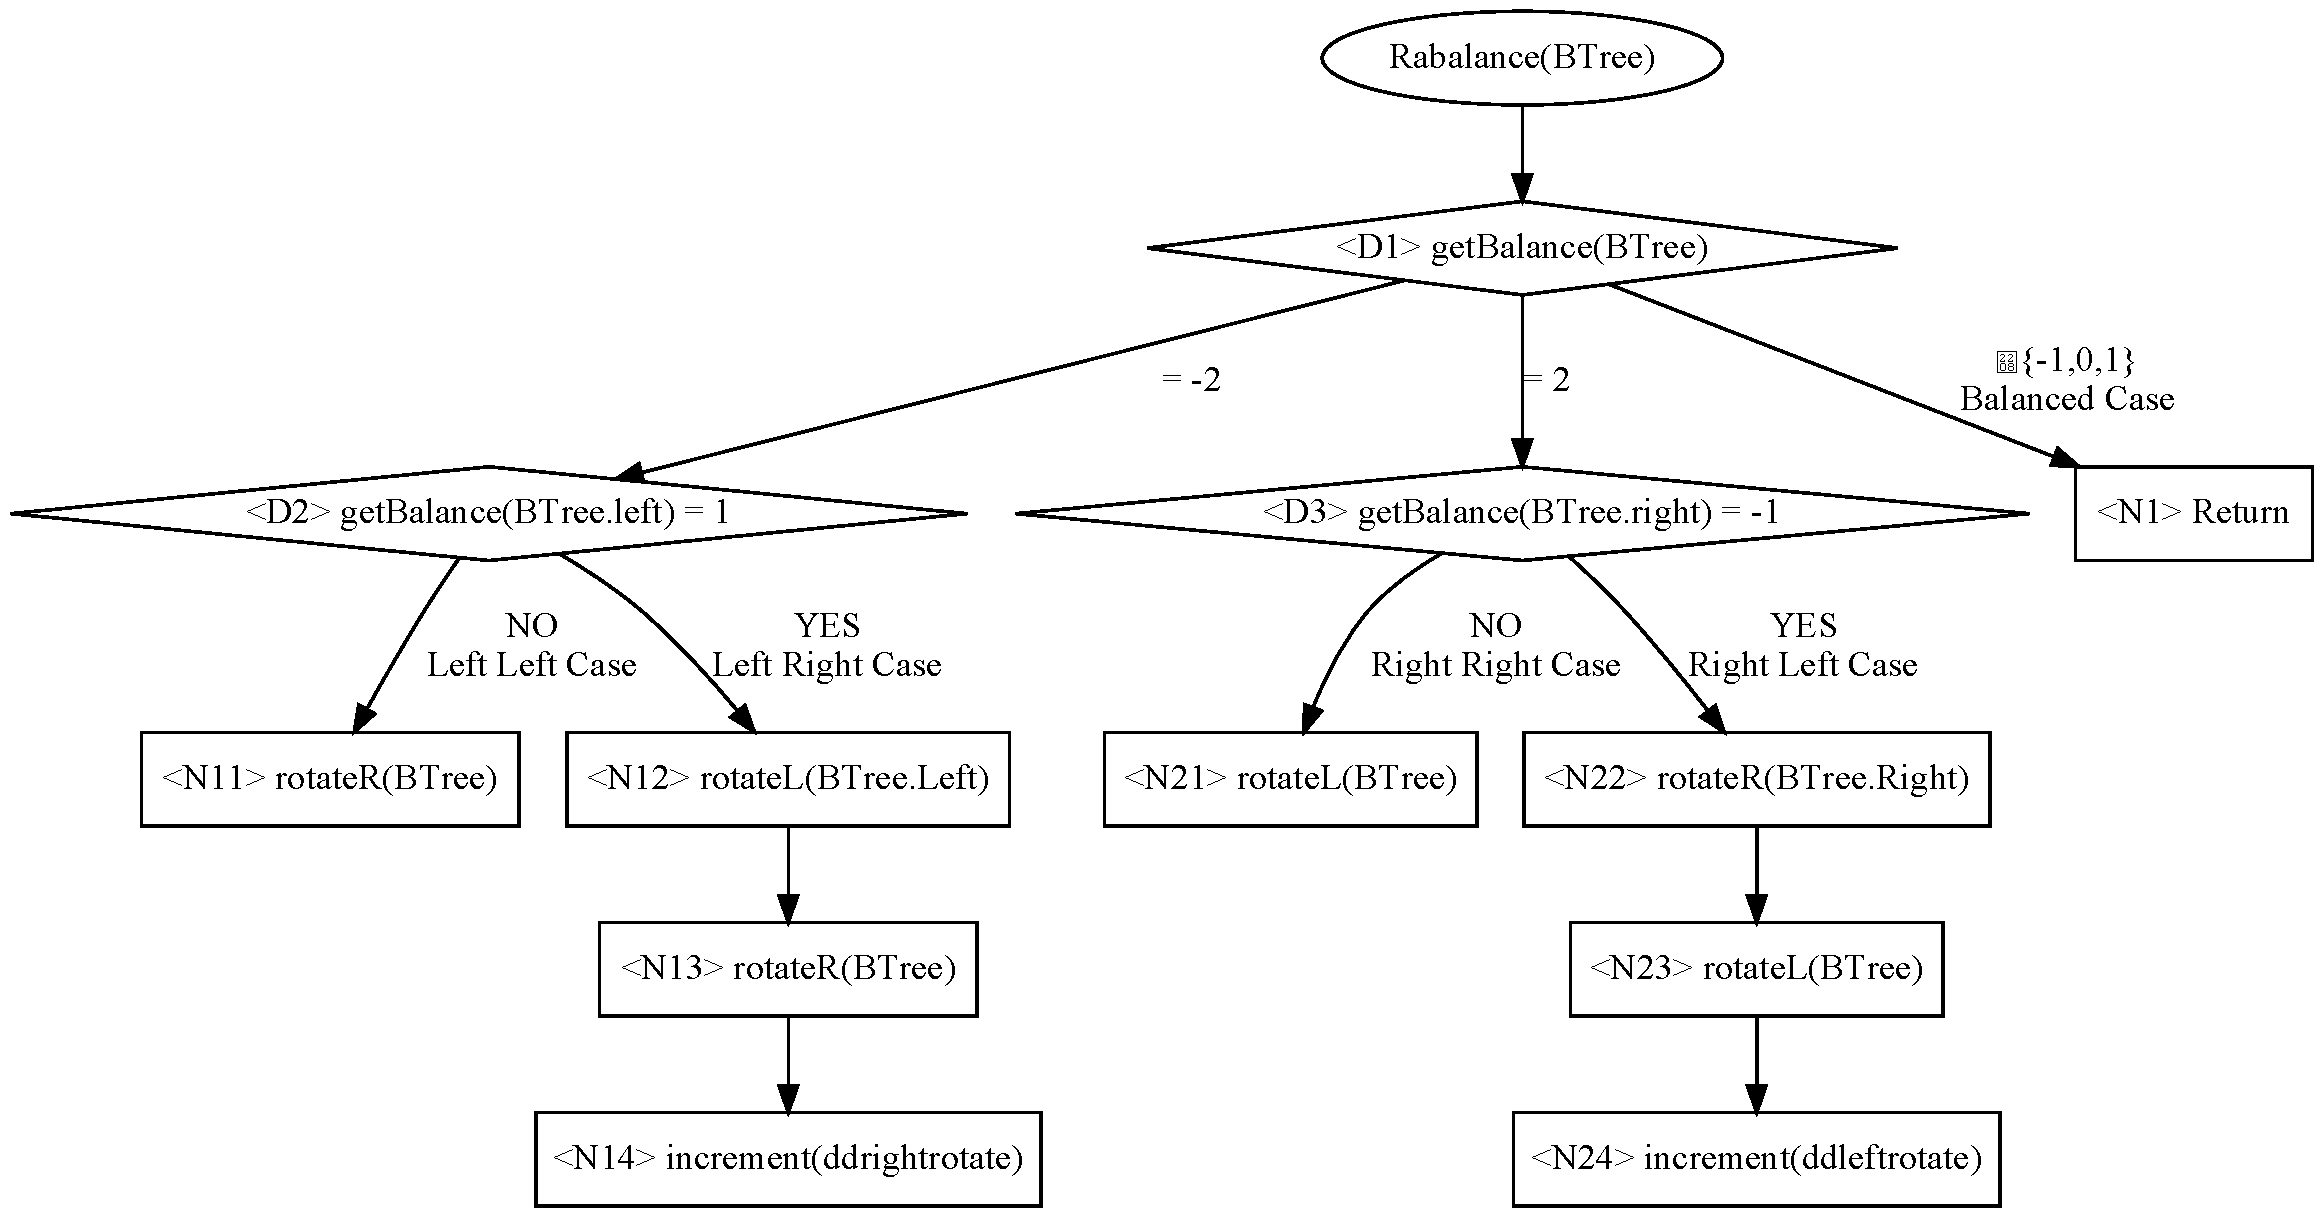
\includegraphics[width = 0.85\textwidth]{img/gv/rebalance}
    \caption{Rebalancierung}
    \label{fig:rebalance}
\end{figure}


\paragraph{Rotate}\label{par:MethodRotate}
Das Rotieren wurde in Abschnitt \nameref{par:rotating} dargestellt.
In Abbildung~\ref{fig:rotate} wird die Rechts- und Linksrotation zusätzlich in jeweils einem
Flussdiagramm dargestellt.
\begin{figure}[hbtp]
    \centering
    \subfloat[\centering Links]{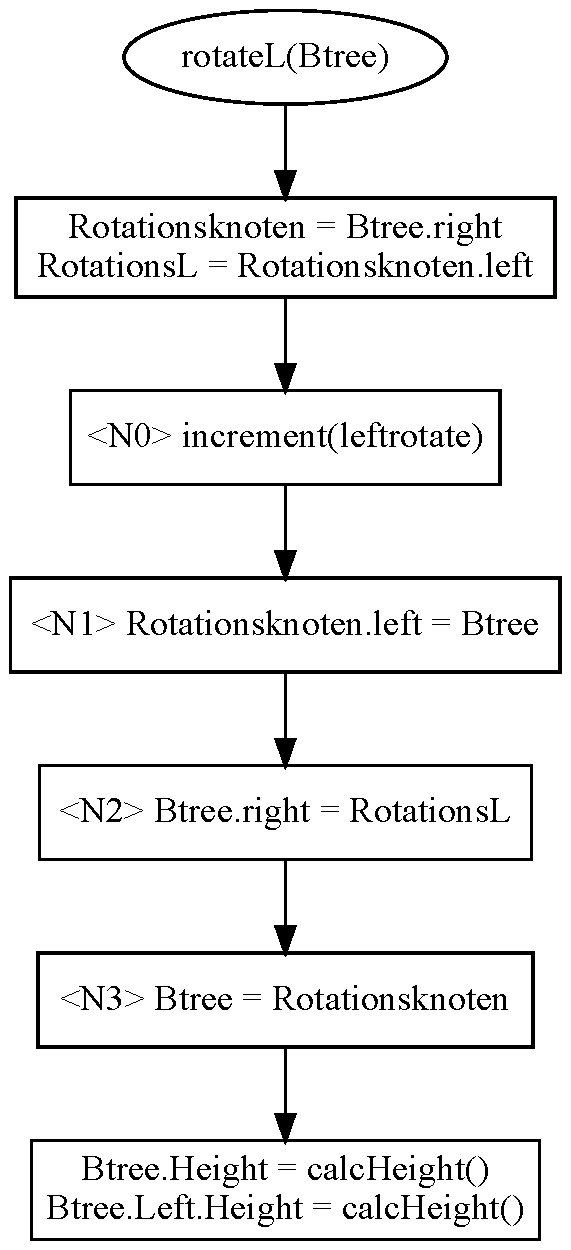
\includegraphics[width = 0.25\textwidth]{img/gv/rotateL.pdf}}
    \subfloat[\centering Rechts]{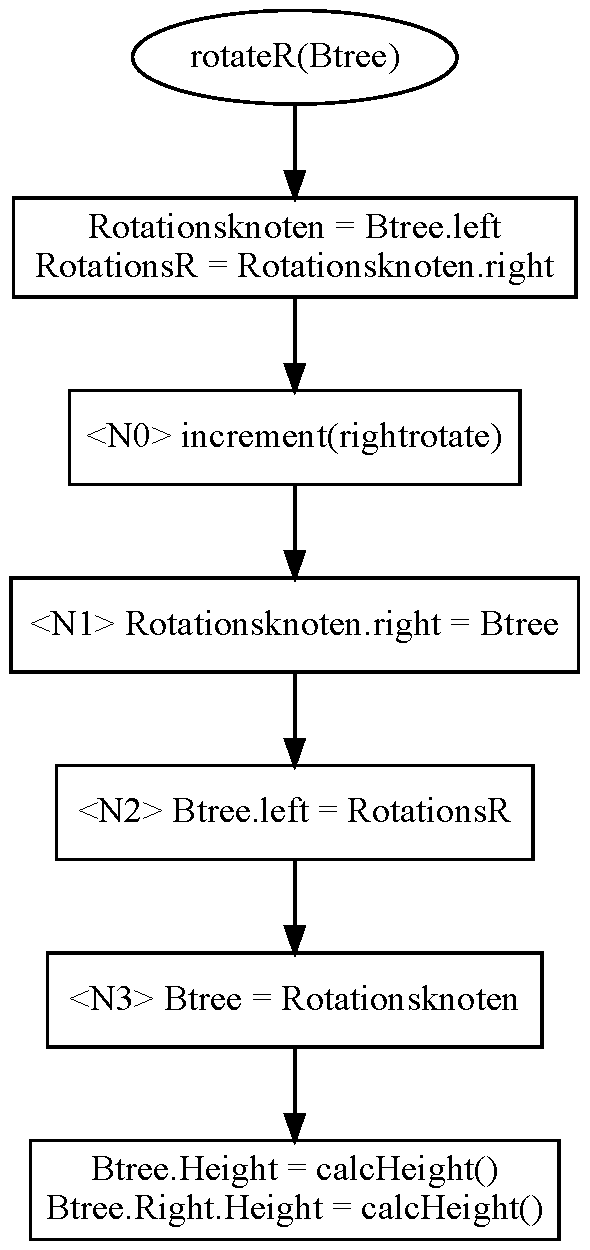
\includegraphics[width = 0.25\textwidth]{img/gv/rotateR.pdf}}
    \caption{Rotieren}
    \label{fig:rotate}
\end{figure}

\FloatBarrier
\subsection{Aufgaben}\label{subsec:aufgaben}

\paragraph{Aufgabe 1.4:}
Beispielhafte Bäume werden mit der zur verfügung gestellten Methode\\
\verb|analyseBT:test(<Anzahl Elemente>)| analysiert.
\subparagraph{100 Elemente}
Ein Aufruf mit 100 Elementen ergibt folgende Ausgabe:
\begin{verbatim}
>analyseBT:test(100).
Bei gegebener Höhe 8:
         minimale Anzahl Knoten: 54.
         maximale Anzahl Knoten: 255
Bei gegebener Anzahl an Knoten 100:
         minimale Höhe: 6.
         maximale Höhe: 9
Durchschnittliche Balancefehler: 0.28
         maximaler Balancefehler: 1.
\end{verbatim}

An der Ausgabe ist zu erkennen, dass der erzeugte Baum mit 100 Elementen eine Höhe von 8
aufweist.
Dies liegt innerhalb des theoretischen Rahmens für AVL Bäume der Elementanzahl 100 von mindestens
6 und maximal 9.
Die Ausgabe zeigt außerdem die minimale und maximale Elementanzahl für einen Baum der
vorgegebenen Höhe an, die hier bei 54 und 255 liegt.
Der maximale Balancefehler beträgt 1, somit wurde die AVL-Bedingung bei jedem Knoten eingehalten.
Der durchschnittliche Balancefehler beträgt 0.28, somit hatten 28 der 100 Knoten eine Balance
von -1 oder 1.

\subparagraph{1000 Elemente}
Ein Aufruf mit 1000 ergibt folgende Ausgabe:
\begin{verbatim}
>analyseBT:test(1000).
Bei gegebener Höhe 12:
         minimale Anzahl Knoten: 376.
         maximale Anzahl Knoten: 4095
Bei gegebener Anzahl an Knoten 1000:
         minimale Höhe: 9.
         maximale Höhe: 14
Durchschnittliche Balancefehler: 0.321
         maximaler Balancefehler: 1.
\end{verbatim}

Aus der Ausgabe wird ersichtlich, dass die AVL-Bedingung auch bei 1000 Elementen eingehalten wird.
Des Weiteren wird die Logarithmische Natur des AVL-Baumes ersichtlich:
Bei einer Verzehnfachung der Elementanzahl hat sich die Höhe lediglich um dem Faktor 0.5 erhöht.

\subparagraph{Fehlerhafter Baum}
Ein Aufruf mit einem Baum, der an einem Knoten eine Balance von 2 besitzt, ergibt folgende Ausgabe:
\begin{verbatim}
>analyseBT:analyseBT({3, 3, {}, {4, 2, {}, {5, 1, {}, {}}}}).
Bei gegebener Höhe 3:
         minimale Anzahl Knoten: 4.
         maximale Anzahl Knoten: 7
Bei gegebener Anzahl an Knoten 3:
         minimale Höhe: 2.
         maximale Höhe: 1
Durchschnittliche Balancefehler: 1.0
         maximaler Balancefehler: 2.
\end{verbatim}
Der maximale Balancefehler beträgt wie erwartet 2, außerdem liegt die Höhe des Baumes über dem
theoretischen Maximum.
Der Baum ist somit kein AVL-Baum.

\paragraph{Aufgabe 2.5}
Es wird ein Baum aus 100 Zufallszahlen erstellt, anschließen werden zufällig 88 davon wieder
gelöscht.
In Abbildung~\ref{fig:88before} ist der Baum vor dem Löschen zu sehen.
In Abbildung~\ref{fig:88after} ist der Baum nach dem Löschen zu sehen.

\begin{figure}[hbtp]
    \centerline{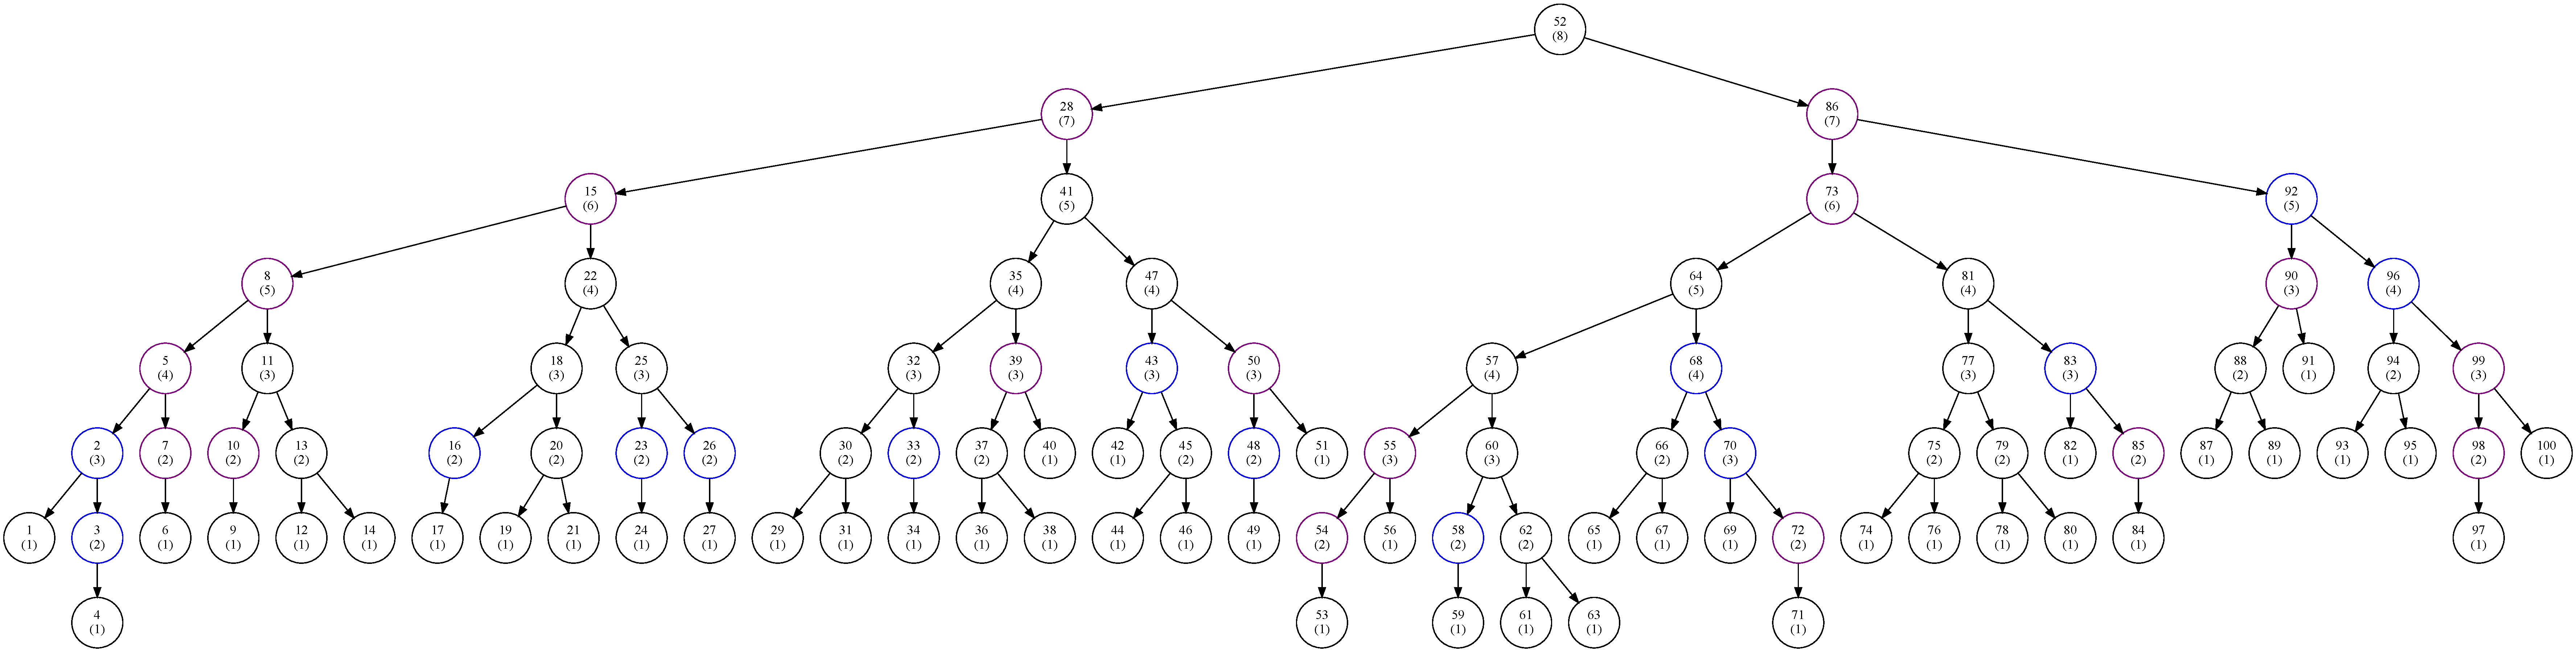
\includegraphics[width = 1.2\textwidth]{img/gv/aufgabe1_6_before.pdf}}
    \caption{Vor dem Löschen}
    \label{fig:88before}
\end{figure}
\begin{figure}[hbtp]
    \centering
    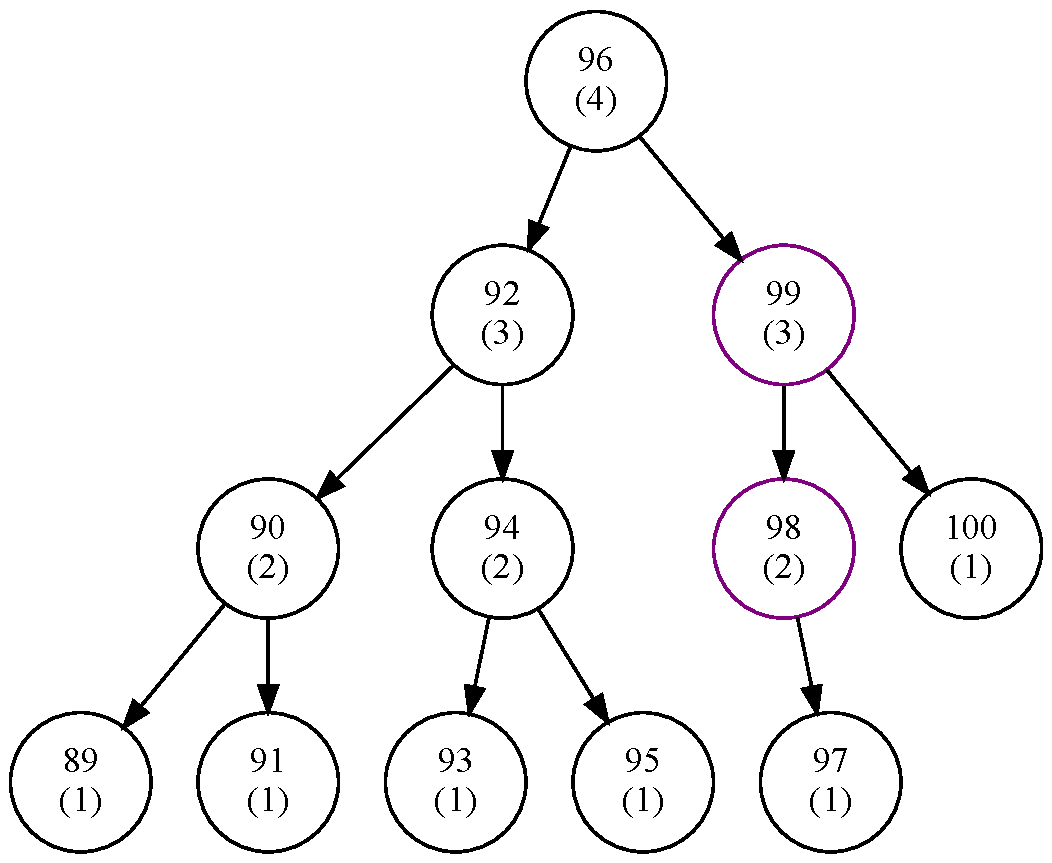
\includegraphics[width = 0.25\textwidth]{img/gv/aufgabe1_6_after.pdf}
    \caption{Nach dem Löschen}
    \label{fig:88after}
\end{figure}
\FloatBarrier

